% Paths assume compilation from the repository root. Use figure* for IEEE two-column layout.
\begin{figure}[t]
  \centering
  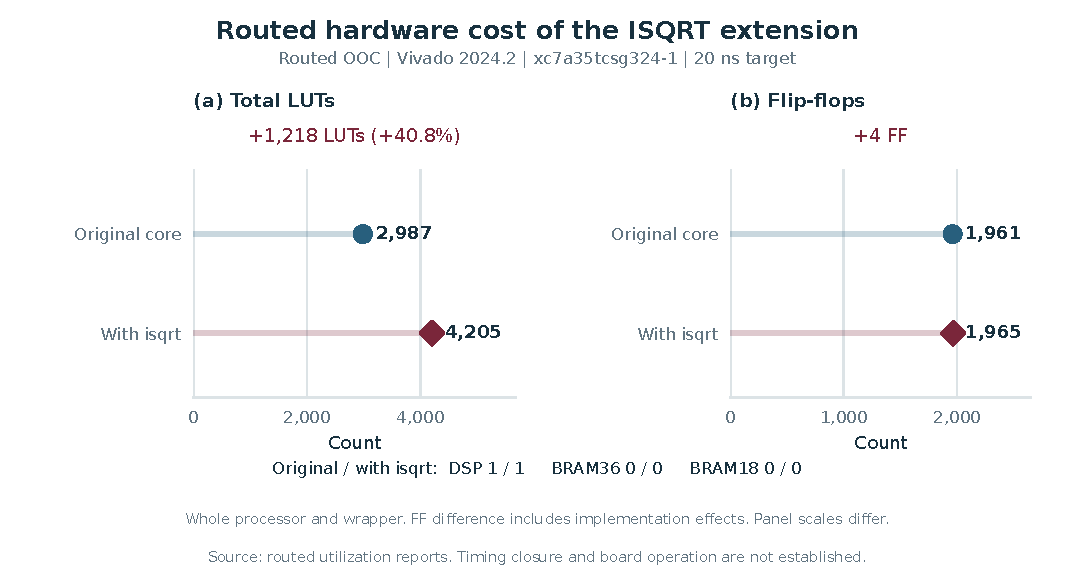
\includegraphics[width=\linewidth]{output/pdf/fig09_routed_resources.pdf}
  \caption{Whole-design resource utilization after out-of-context placement and routing. Counts and the relative LUT increase come from the top-level utilization rows and include the wrapper. Panel scales differ. The mapped FF difference includes implementation effects and does not imply an added RTL pipeline stage. Both designs use the existing multiplier DSP and no BRAM. These runs do not establish complete physical timing closure.}
  \label{fig:fig09_routed_resources}
\end{figure}

\begin{figure}[t]
  \centering
  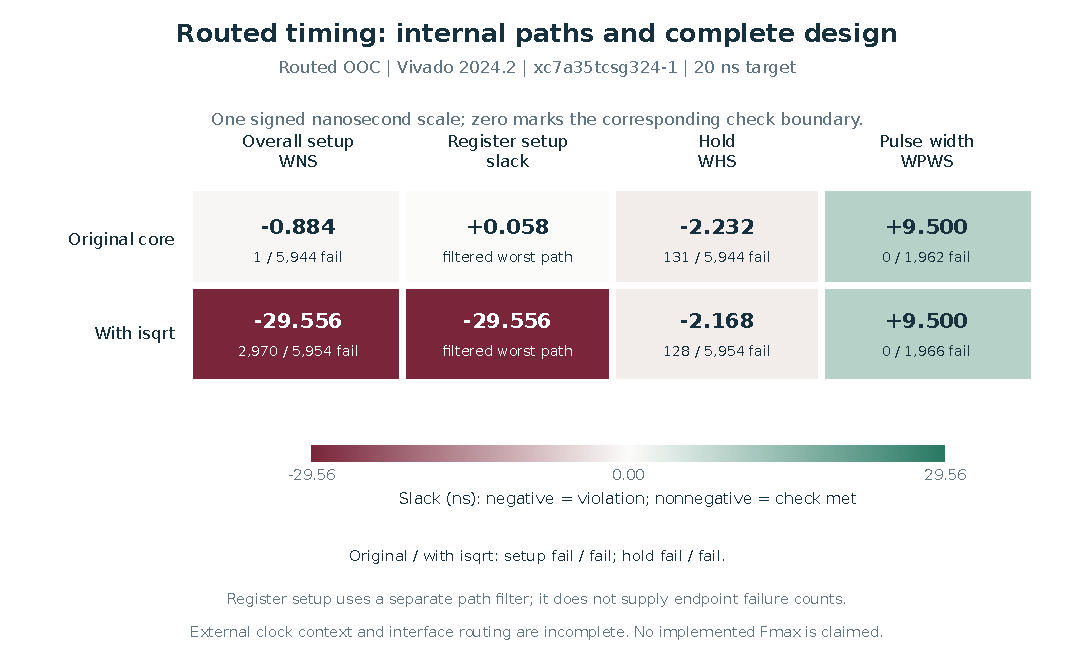
\includegraphics[width=\linewidth]{output/pdf/fig10_routed_timing.pdf}
  \caption{Routed OOC slack heatmap at a 20 ns clock target. Overall setup, hold and pulse-width cells use the complete design timing summaries and show failing/total endpoints. The register-setup column shows the worst path from a separate register-to-register query; endpoint failure counts are not available for that filtered query. All cells share one signed nanosecond scale centered on zero. A nonnegative filtered register setup slack does not establish complete timing closure. External clock context and interface routing remain incomplete.}
  \label{fig:fig10_routed_timing}
\end{figure}

\begin{figure}[t]
  \centering
  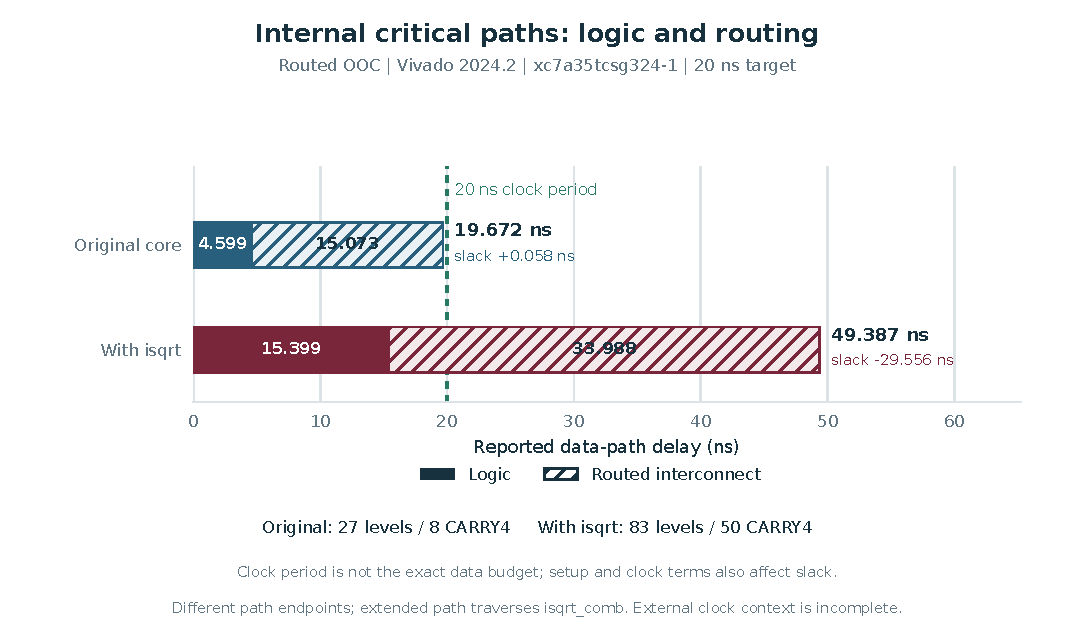
\includegraphics[width=\linewidth]{output/pdf/fig11_routed_path_delay.pdf}
  \caption{Logic and routed interconnect contributions to each design's worst reported internal register setup path. Delay segments and totals are read from the reports. The extended path traverses isqrt\_comb. The 20 ns reference is the clock period, not the exact available datapath budget; slack also includes register setup and clock terms. The paths have different endpoints. These delays cover complete selected paths and do not isolate the square-root block. External clock context remains incomplete.}
  \label{fig:fig11_routed_path_delay}
\end{figure}

\begin{figure}[t]
  \centering
  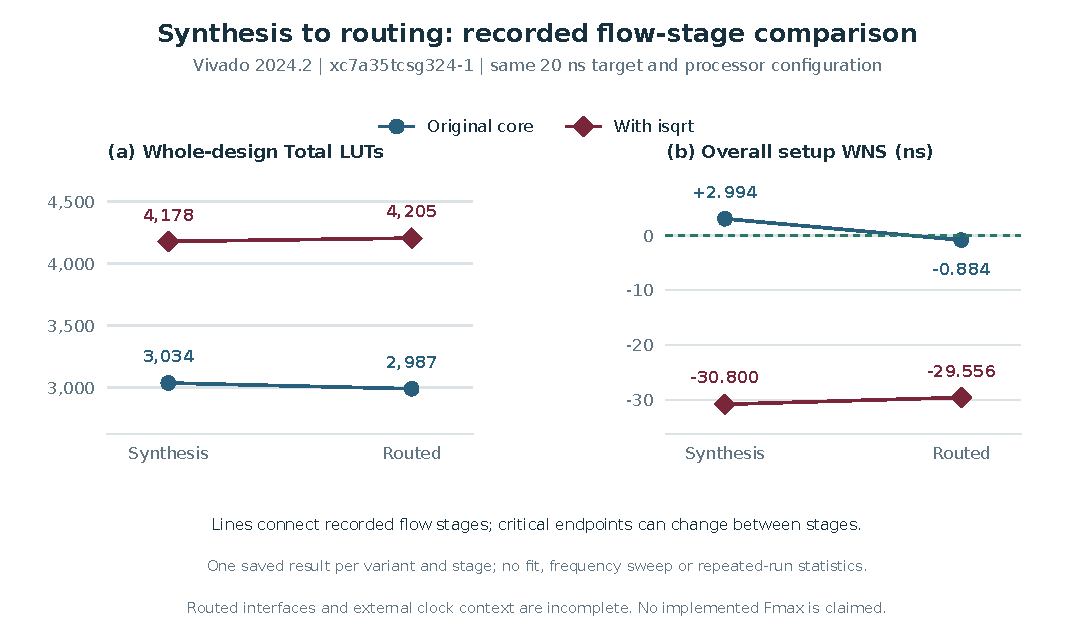
\includegraphics[width=\linewidth]{output/pdf/fig12_fpga_stage_comparison.pdf}
  \caption{Recorded synthesis and routed OOC results for the original and extended cores. Each line connects two saved flow stages, with direct numerical labels. The left panel shows whole-design Total LUTs; the right shows complete-design setup WNS. Connections indicate flow order, not a fitted trend, frequency sweep or repeated-run distribution. Critical endpoints can change between stages. Interface and external clock context remain incomplete. No implemented Fmax or power is claimed.}
  \label{fig:fig12_fpga_stage_comparison}
\end{figure}
